\chapter{Stanowisko badawcze}
\label{sec:test_stand}

\section{Założenia konstrukcyjne}
\label{sec:stand_assumptions}

Konstrukcji stanowiska badawczego postawiono następujące wymagania:
%lista punktowana
\begin{itemize}
\item prostota budowy,
\item \textbf{powtarzalność warunków pomiarów} - możliwość wielokrotnego wykonania 
próby z jednakową energią uderzenia w przetwornik piezoelektryczny,
\item separacja zewnętrznych czynników mogących mieć wpływ na przebieg odpowiedzi 
elektrycznej,
\item możliwość łatwej wymiany modelu przetwornika (patrz: Rys.\ref{fig:test_stand}),
\item łatwa zmiana mocowania przetwornika,
\item możliwość regulacji energii i pędu wymuszenia mechanicznego w zakresie
 \textbf{$E = 0.24\div14.4$} oraz \textbf{$p = 0.12\div4.8$} obliczonym na podstawie 
 zależności na pęd i energię kinetyczną z fizyki klasycznej \ref{eq:kinetic_energy}.
\end{itemize}

\begin{equation}
E_{s} = \frac{m_{s} \cdot v_{s}^2}{2}
\label{eq:kinetic_energy}
\end{equation}

\begin{equation}
p_{s} = m_{s} \cdot v_{s}
\label{eq:inertia}
\end{equation}
,gdzie: $ m_s$ - masa źródła, $v_s$ - prędkość źródła, $E_s$ - energia kinetyczna źródła, $p_s$ - pęd źródła.

Po podstawieniu danych zawartych w \ref{sec:assumptions} do zależności 
\ref{eq:kinetic_energy} oraz \ref{eq:inertia} otrzymano odpowiednio:

%\begin{equation}

$$E_{smin} = \frac{m_{smin} \cdot v_{smin}^2}{2}=\frac{{0.03}\cdot4^2}{2} = {0.24} mJ$$
\\$$p_{smin} = m_{smin} \cdot v_{smin} = {0.03}\cdot 10^{-3} \cdot 4 = {0.12} \cdot 10^{-3}\frac{kg \cdot m}{s^2}$$
\\$$E_{smax} = \frac{m_{smax} \cdot v_{smax}^2}{2}=\frac{0.80\cdot6^2}{2} = 14.4 mJ$$
\\$$p_{smax} = m_{smax} \cdot v_{smax} = 0.80 \cdot 6 = 4.8 \cdot 10^{-3} \frac{kg \cdot m}{s^2}$$

%\end{equation}

\section{Projekt stanowiska}
\label{sec:stand_project}

\indent
Biorąc pod uwagę powyższe założenia zdecydowano o zastosowaniu napędu sprężynowego 
w projektowanym stanowisku. Z tego powodu rozpoczęto pracę od doboru sprężyny. 
Głównymi kryteriami doboru były wpółczynnik sprężystości sprężyny oraz jej długość. 
Na podstawie zależności \ref{eq:spring} Wybrano sprężynę o $k=0.17\frac{N}{mm}$ 
i długości $l=80mm$. Następnie zaprojektowano
\footnote{Szczegółowy projekt stanowiska dostępny pod 
\href{http://www.google.com}{adresem}}%TODO
układ przedstawiony na Rys.\ref{fig:test_stand}. Element symulujący źródło impulsu 
mechanicznego (w dalszej części pracy dla uproszczenia przyjmuje się nazwę \textbf{ciało M})
przewidziano wykonać z drewnianej sklejki o masie $m_s = 3.60g$.

\begin{figure}[htbp]
\centering
\includegraphics[width=\linewidth]{pictures/zlozenie_mgr.pdf}
\caption{Projekt stanowiska badawczego.}
\label{fig:test_stand}
\end{figure}

\begin{equation}
E_s = E_p = k \cdot x^2
\label{eq:spring}
\end{equation}
,gdzie: $E_p$ - energia potencjalna sprężystości $k$ - współczynnik 
sprężystości, $x$ - odkształcenie sprężyny.

\indent Tor, po którym porusza się ciało M, zdecydowano się wykonać z konstrukcyjnego 
profilu aluminowego o wymiarach normatywnych \cite{PN_constr}. Podstawą do jego zastosowania nie były
kryteria wytrzymałościowe, lecz rozbudowane możliwości montażu. W opisywanym profilu
zaprojektowano sprężynę, ciało M, przesuwny element regulacyjny naciągu sprężyny 
wraz ze spustem oraz podpory konstrukcji przetwornika. Elementy zaplanowano zamontować 
przy użyciu śrub opisanych w normie \cite{PN_constr}.
Sam profil zamontowano do drewnianej podstawy, wykorzystując takie same śruby. Zastosowanie
powyższego rozwiązania zdecydowanie ułatwia stworzenie stanowiska. Wpływa na to nie tylko
łatwość montażu, ale również dostępność zastosowanych materiałów i półfabrykatów.


\section{Realizacja i charakterystyka stanowiska}
\label{sec:stand_realization}

Na rys.\ref{fig:test_stand_photo} przedstawiono realizację 
projektu opisanego w \ref{sec:stand_realization}. Realizacja nieco różni się od
rysunku projektowego. Główną rożnicę stanowi kształt podstawy. Powodem było ułatwienie
montażu modelu przetwornika piezoelektrycznego oraz stateczność stanowiska. 

\begin{figure}[htbp]
\centering
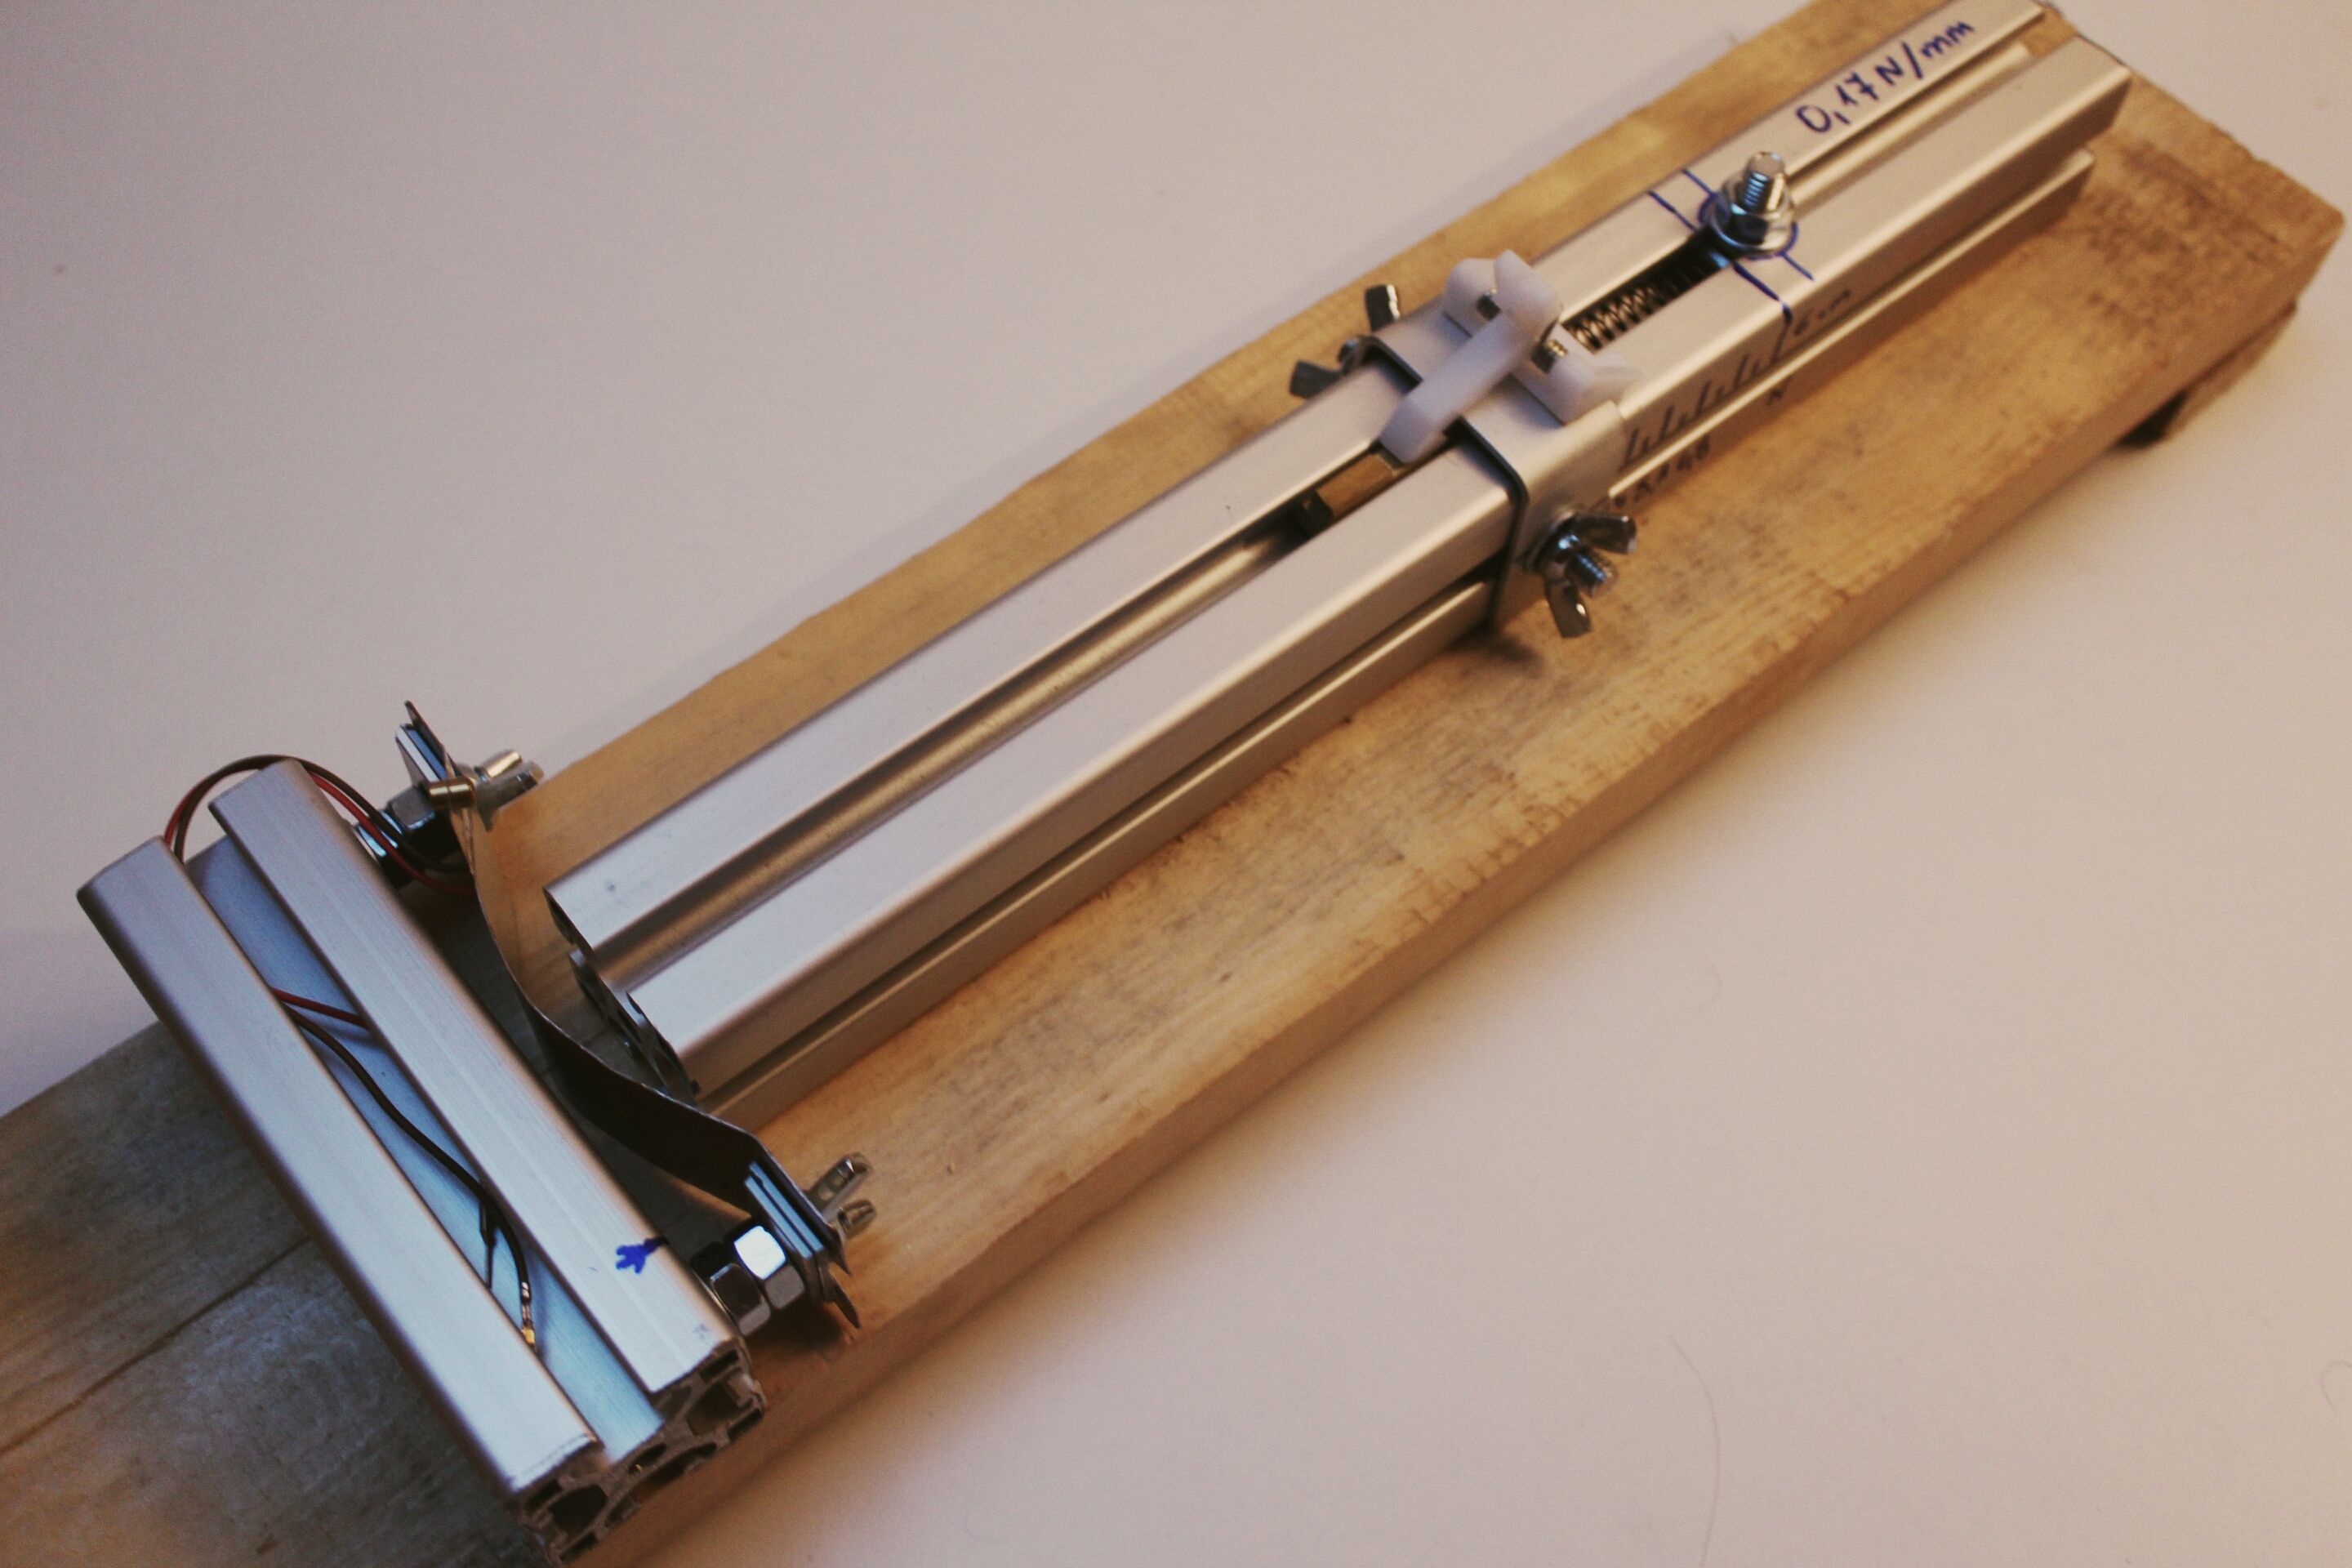
\includegraphics[width=\linewidth]{pictures/lab_stand.jpg}
\caption{Realizacja stanowiska badawczego.}
\label{fig:test_stand_photo}
\end{figure}

Tak skonstruowany układ laboratoryjny pozwolił uzyskać charakterystyki mechaniczne 
$E_C(x)$ i $p_C(x)$ przedstawione na Rys.\ref{fig:mech_char}. 
Gdyby wziąć pod uwagę możliwość wymiany sprężyny
oraz elementu wprawianego w ruch otrzymanoby całą rodzinę charakterystyk, a przez to
większą uniwersalność urządzenia. Zależności opisujące $E_C$ oraz $p_C$ zaprezentowano
przy pomocy wzorów \ref{eq:crash_energy} i \ref{eq:crash_inertion}


\begin{equation}
  E_C = E_k - W
  \label{eq:crash_energy}
\end{equation}
  ,gdzie: $E$ - energia kinetyczna przed zderzeniem, 
  $E_C$ - energia kinetyczna na początku ruchu,
  $W$ - straty energii na tarcie podczas ruchu.

\begin{equation}
  p_C = m \dot v_C^2
  \label{eq:crash_inertion}
\end{equation}
  ,gdzie: $v_C$ - prędkość ciała przed zderzeniem, 
  $p_C$ - pęd ciała przed zderzeniem,
  $W$ - straty energii na tarcie podczas ruchu.


\pgfplotsset{width=\linewidth,compat=1.3}

\begin{figure}[htbp]
\centering
    \begin{tikzpicture}
%    \pgfplotsset{
%    scale only axis,
%    scaled x ticks=base 10:3,
%    xmin=0, xmax=0.06
%}
      \begin{axis}[
          width=\linewidth, % Scale the plot to \linewidth
          grid=major, % Display a grid
          grid style={dashed,gray!30}, % Set the style
          xlabel=${\delta}x$ , % Set the labels
          ylabel=$E_C$,
          x unit=\si{\milli\metre}, % Set the respective units
          y unit=\si{\milli\joule},
          ymin = 0,
          xmin = 0,
          ]
          \addplot[smooth,mark=*,blue] table[x=x,y=E-W,col sep=comma] {pomiary.csv};
          \label{plot_one}
          \addlegendentry{Energia przed zderzeniem}
          \legend{}
        \end{axis}
        
        
        \begin{axis}[
          axis y line*=right,
          axis x line=none,
          width=\linewidth, 
          ylabel=$p$,
          y unit=\si{\k\g\m\per\square\s},
          ymin = 0,
          xmin = 0,
          legend style={at={(0.5,-0.2)},anchor=north},
        ] 
        \addlegendimage{/pgfplots/refstyle=plot_one}
        \addlegendentry{Energia przed zderzeniem}
        \addplot[smooth,mark=x,red] table[x=x,y=p,col sep=comma] {pomiary.csv};
        \addlegendentry{Pęd przed zderzeniem}
      \end{axis}
    \end{tikzpicture}
\caption{Charakterystyka mechaniczna stanowiska badawczego.}
\label{fig:mech_char}
\end{figure}


